\documentclass[12pt]{article}
\usepackage[margin=1in]{geometry}
\usepackage{amsmath}
\usepackage{amssymb}
\usepackage{fancyhdr}
\usepackage{pgfplots}
\usepackage{graphicx}
\usepackage{enumitem}
\usepackage{hyperref} 
\pgfplotsset{compat=1.16}


\author{Zhijie Xia, Yuan Liu, Zixing Wei, G-69}
\title{CPSC 471 Final Report}


\pagestyle{fancy}
\renewcommand{\headrulewidth}{0pt}
\renewcommand{\footrulewidth}{0pt}


\fancyhf{}
\rhead{
    Final Report
}
\rfoot{
    Page \thepage
}

\begin{document}
\maketitle
\newpage

\textbf{Abstract:}

\vspace*{5mm}
“YourStore” is a non-profit online shopping platform. Aside from its non-profit nature, its functionality is very similar to a retailer’s online shopping website, for example, Best Buy and its bestbuy.ca. It provides small stores a website application that is easy to configure and maintain.
The store owners will be given the permission to list other products, change the inventory, and track all the placed orders. All end users’ data (products, orders, inventories) will be stored in the database that can be accessed and modified when needed. The project’s core concept is providing an opportunity to store owners to sell their
products online, which is realized by a series of core functions, such as customers’ order placement, local stores’ order acceptance and arrange delivery . Order status is also updated at different stages of the order and tracked by all end-users.
Our project has similar functionalities to other commercial online shopping services. It facilitates a complete process of shopping order, realized by many core functions, such as customers’ order placement, sellers’ order acceptance and shipment. Order status is also updated at different stages of the order and tracked by all end-users. All CRUD (create, read, update and delete) functions can be realized via Postman, and our mobile-friendly web app can also visualize the entire user-flow from registration to order complete.
“YourStore” is made with React framework, Redux, Node.js, MongoDB, Express. With Node.js MongoDB, and Express, we were able to develop back-end API in javascript language to implement all necessary CRUD functions, as well as connect our back-end API to a mobile-friendly front-end web app, which is developed with a combination of React, Redux, Bootstrap. All API endpoints are properly connected to our database.


\newpage
\textbf{Introduction:}
\vspace*{5mm}

Since the prolonged pandemic has forced people to increasingly move their works and life online, many small sized 
local stores are suffering a plummeting in the number of in store shoppers. Thus, they desire to seize the opportunity to develop online businesses like other large-chain retail stores. This problem is partially solved by online workshops like Amazon, Ebay, and StockX. 
Their business model allows business owners to sell other products on their website by charging a substantial percentage of commission. Since the pandemic has lasted for a long time and there is no sign of an end at present, many local small-sized store owners argue the current business model that they build on the online platforms becomes less economically viable and not commercially sustainable for them when a considerable part of their revenue is being taken by the platform provider.

\vspace*{10mm}

\textbf{Our System:}
\vspace*{5mm}

"YourStore" is a non-profit online shopping platform. Aside from its non-profit nature, its functionality is very similar to a retailer’s online shopping website, for example, Best Buy and its bestbuy.ca. It provides small stores a website 
application that is easy to configure and maintain. The store owners will be given the permission to list other products, change the inventory, and track all the placed orders. All end users, data (products, orders, inventories) will be stored 
in the database that can be accessed and modified when needed. The project’s core concept is providing an opportunity to store owners to sell their products online, which is realized by a series of core functions, such as customers' order placement, local stores' 
order acceptance and arrange delivery . Order status is also updated at different stages of the order and tracked by all end-users.

\newpage 
\textbf{Project Design Description:}

We have three types of users : \textbf{customer}, \textbf{seller}, and \textbf{administrator}. Each type of user needs to 
login first and receive an access token for future interactions with APIs. Note that \textbf{administrator} users 
are predefined and an user cannot register himself/herself as a type of \textbf{administrator}.
\vspace*{5mm}

\textbf{Customer:}
    After a \textbf{customer} user logs in, he/she would be given a search bar which has a dropdown menu of category and a text input 
    field. 
    
    The customer can choose a particular category from the categories or "All" and search products with the text input. After clicking "Search",
    the page would redirect customer to search results, a list of products that meet the searching conditions would be showed on the screen.
    
    The products would be showed with their descriptions, images, prices and inventories information so that the customer can carefully exam.
    
    After the customer decides what products he/she may want, he/she can choose to add the products by clicking "Add To Cart" button, and the product information 
    would be added into his/her cart. 
    
    When the customer decides to checkout, he/she would goes to his/her cart page, and the list of products that the 
    customer added would show on the screen. 
    
    The customer may want to delete some unwantted products by clicking the trashbin icon, thus the product would be 
    remove from his/her cart. 
    
    In order to create orders and actually purchase the products in the cart, the customer must supply a receiver name 
    and a receiver address to create orders. The receiver name and address would be stored in the database so that the seller can arrange shipping when the order 
    is paid for. 
    
    After creating the products, the customer needs to goto his/her "Orders" page where he/she can find a list of all orders of his/her and do 
    some actions, for example, "Pay" for the order or "Cancel" the order. While waiting for the products to arrive, the customer can follow the status in his/her
    order pages. 

\vspace*{5mm}
\textbf{Seller:} After a \textbf{seller} user logs in, he/she would be redirected to a page where he/she can find 
all his/her products that are listing in the site for sell. 

If there are any products that the seller wants to sell, 
he/she can click "Add New Product" buttons, a modal input form would pop up. The seller must fill in the product details 
in all blank fields and click "Create Product" to insert the product information in the database so that a customer can find 
the product in the search result and potentially add it into the cart and purchase it.

Moreover, when the seller can closely mointor the product information especially the inventory status. The seller would want
to add more inventory when he/she has more products avaiable arrived in stock. Or the product want to increase/decrease price of a 
particular product. Maybe he wants to change the description to attract more customers. All the updations can be done in the "My Products" page.

The seller can also see the list of orders that he/she is getting, and the status of the orders(unpaid, paid, unshipped, shipped) to plan the shipment.
Both the seller and the customer of a order would have the same view on the status. When the customer paid for the order, the seller of the 
order can now upload shipping label and complete the order.


\vspace*{5mm}
\textbf{Administrator:}

    The \textbf{administrator} manages every part of the site, and a administrator user has absolutely full permissions to anything, for example, delete 
    a user, delete a product, cancel a order.

    Thus, the administrator account should be carefully protected and given to trusted ones.




\newpage 
\textbf{Project Design EER:}

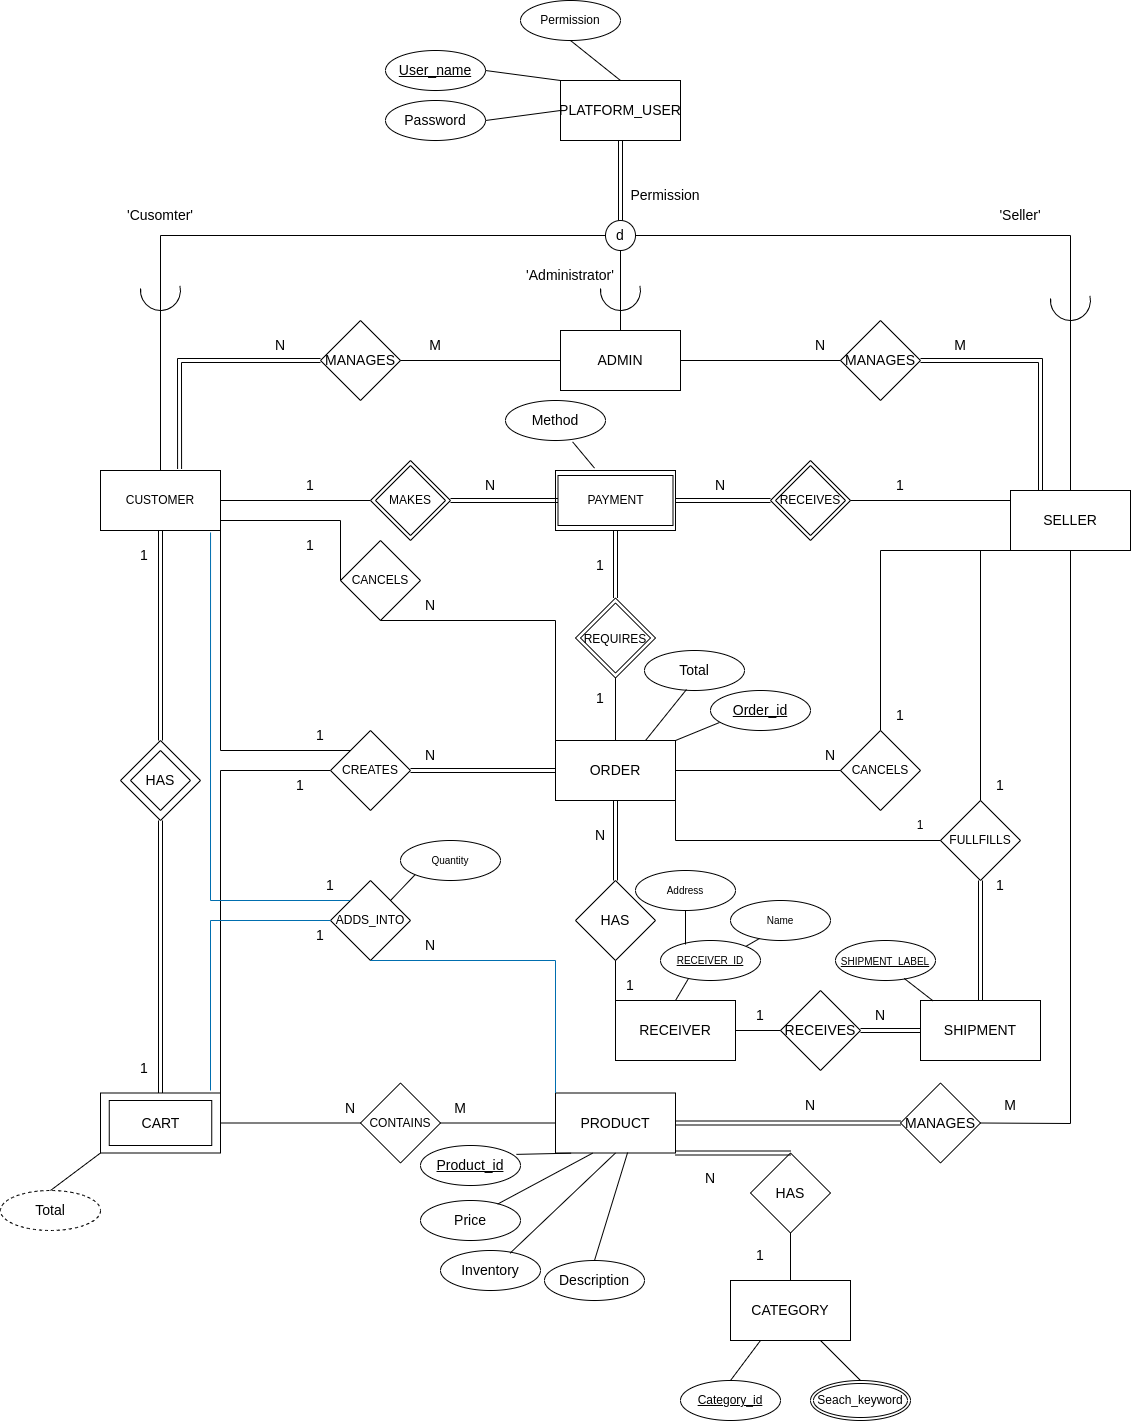
\includegraphics[height=.80\textheight]{Diagrams/onlineShopping_revised.png}

\newpage
\textbf{Implementation RMD:}
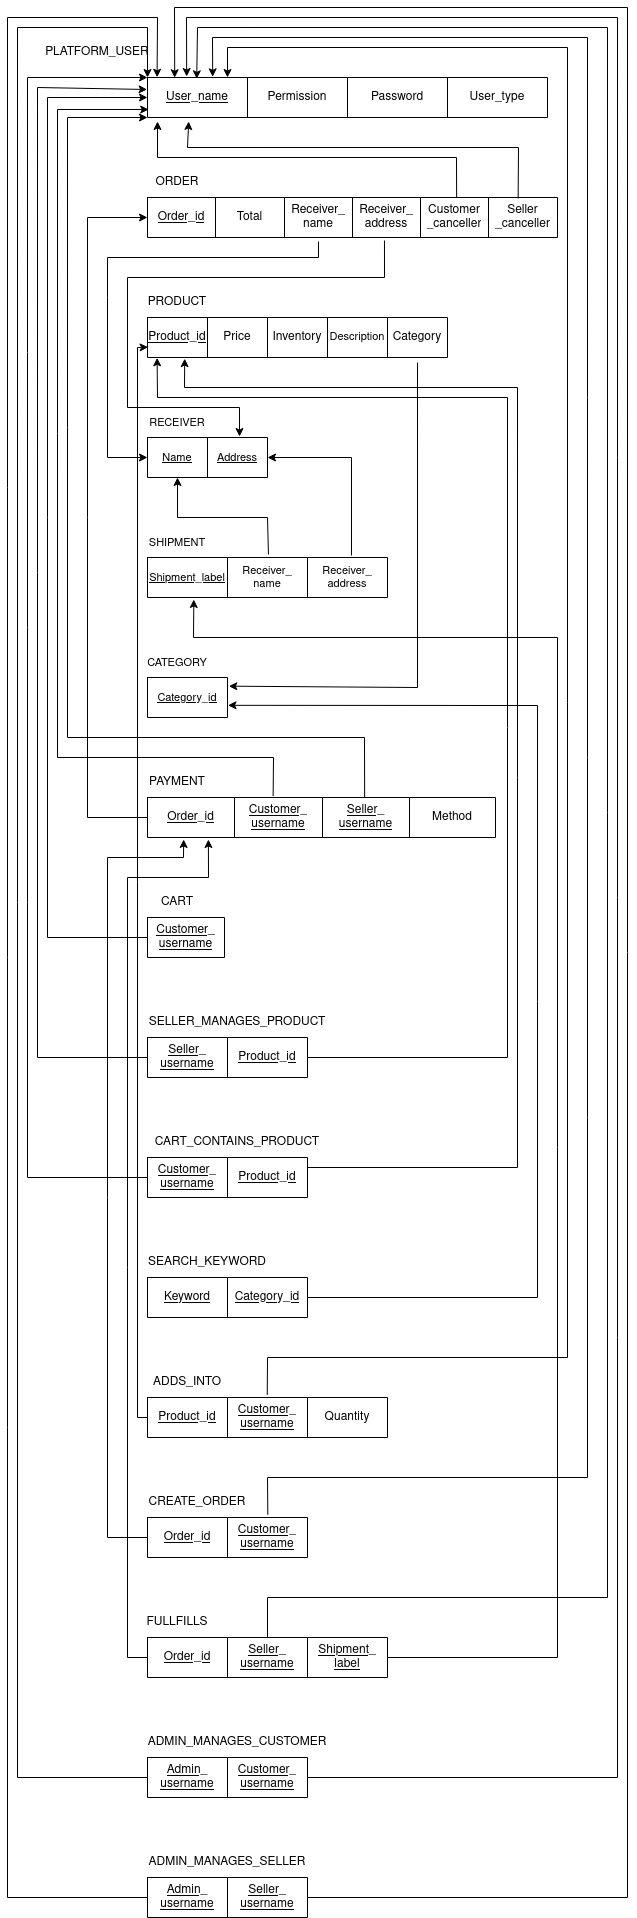
\includegraphics[height=.98\textheight]{Diagrams/relation.png}

\newpage 
\textbf{Implementation DBMS:}

    We have chosed \textbf{MongoDB} as our DBMS. MongoDB is an open source NoSQL database program
    that stores JSON-like documents.


    












\newpage

\textbf{Postman Docuementation:}

\begin{center}
    https://documenter.getpostman.com/view/20517678/Uyr4LftC
\end{center}

\newpage 
\textbf{User Guide:}

\vspace*{5mm}
\textbf{1: Sign in as admin}

Fill in user name as “SuperUser” and password “sodu”. Then click “Login”.

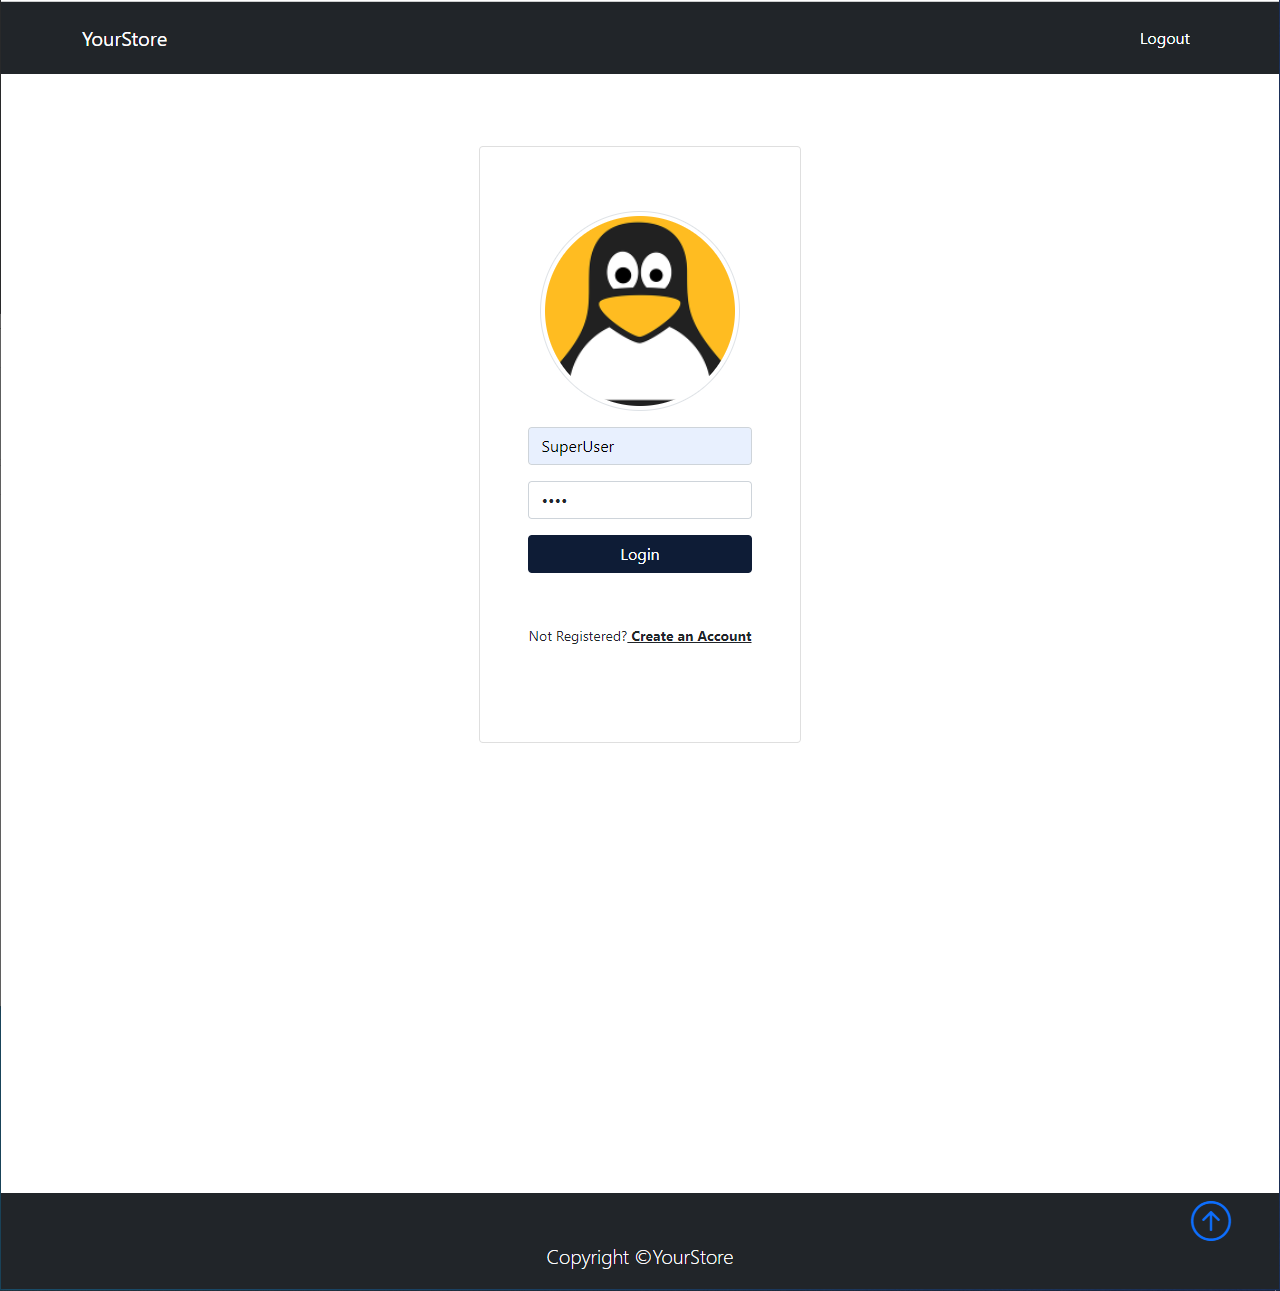
\includegraphics[width=0.45\textwidth]{UserGuideImage/1.png}
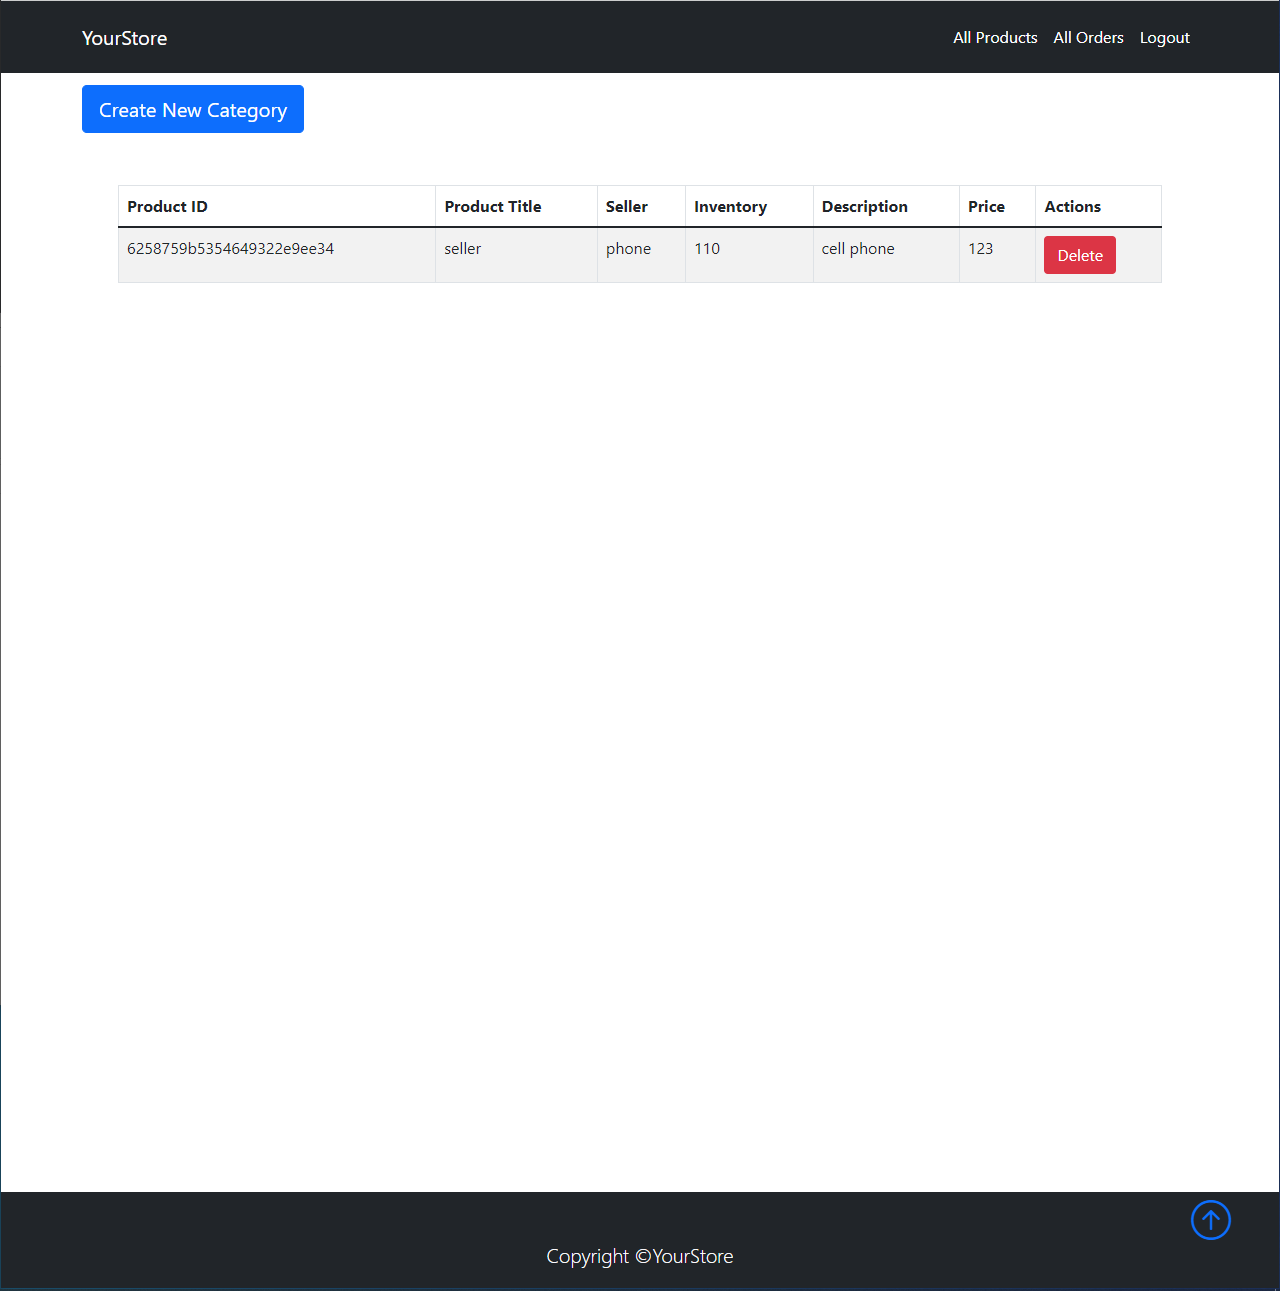
\includegraphics[width=0.45\textwidth]{UserGuideImage/2.png}

\vspace*{5mm}
\textbf{2: Admin manage products}

\hspace*{5mm}\textbf{2.1: Create a new category}

You can access “All Products” page by automatically sign in as admin or click “All Products”
at nav bar. In “All Products” page, admin can create a new category as below.

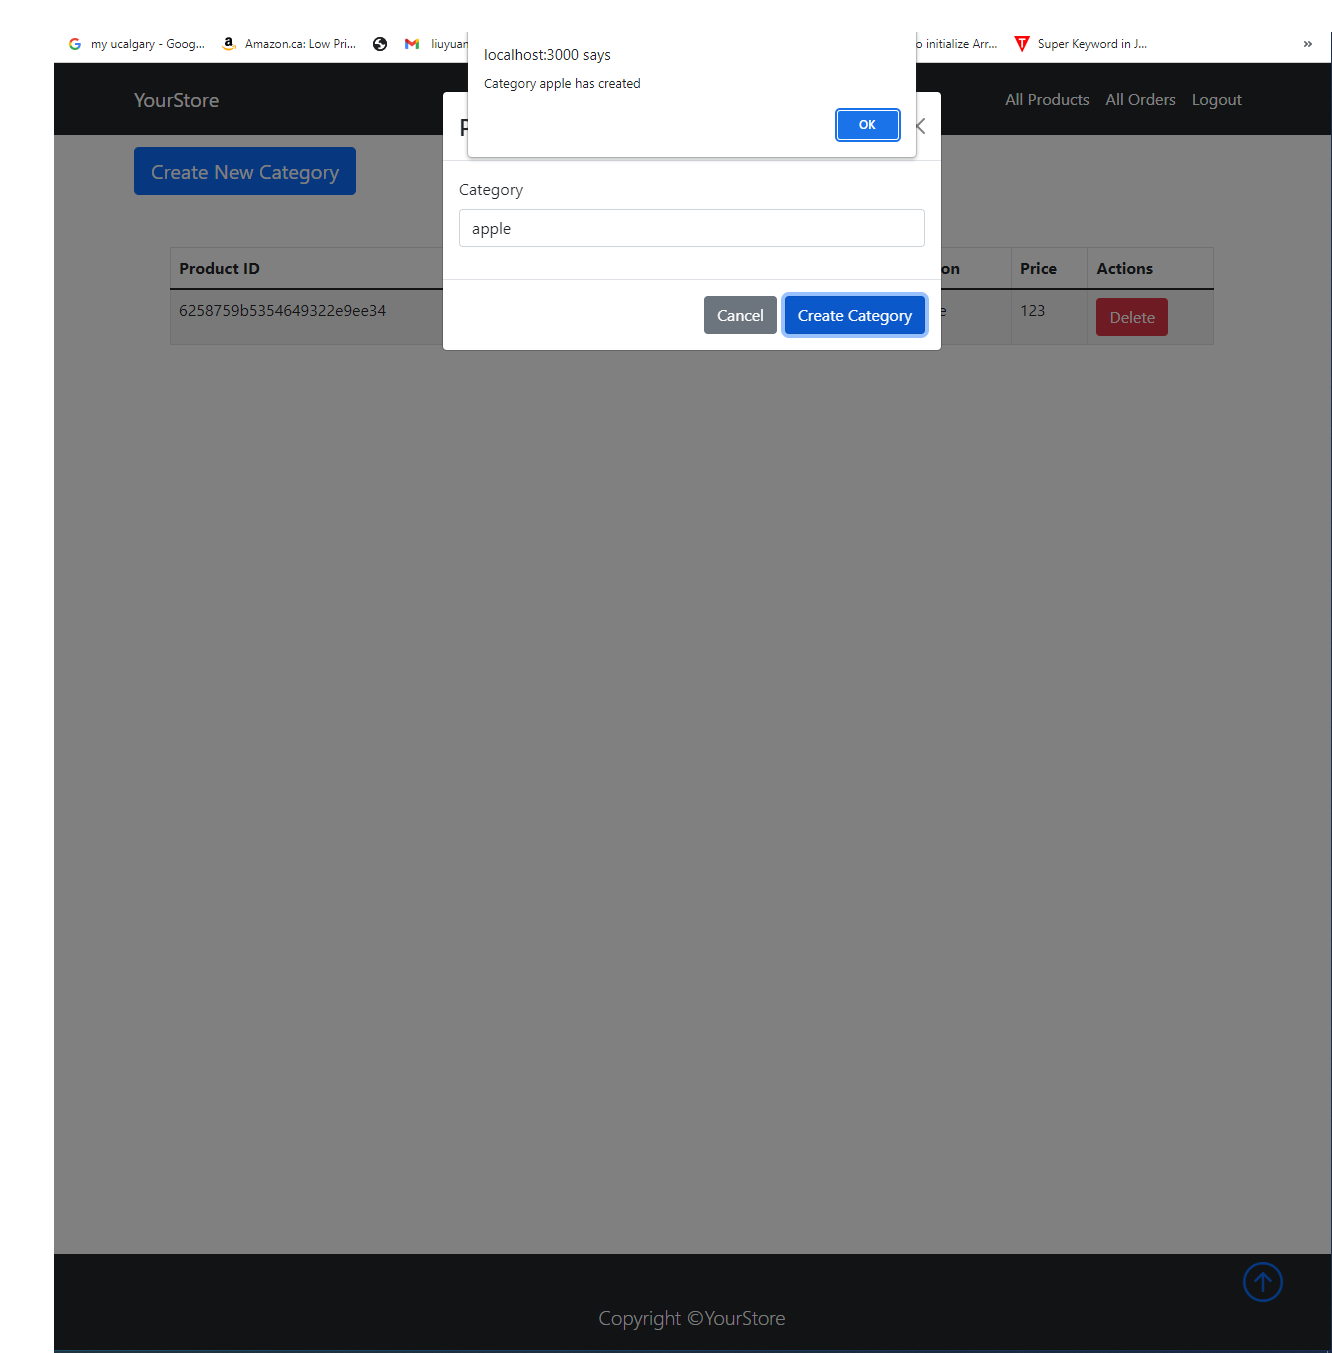
\includegraphics[width=0.45\textwidth]{UserGuideImage/3.png}

\newpage
\hspace*{5mm}\textbf{2.2: Delete products}

In “All Products” page, admin can delete any existing products as below.

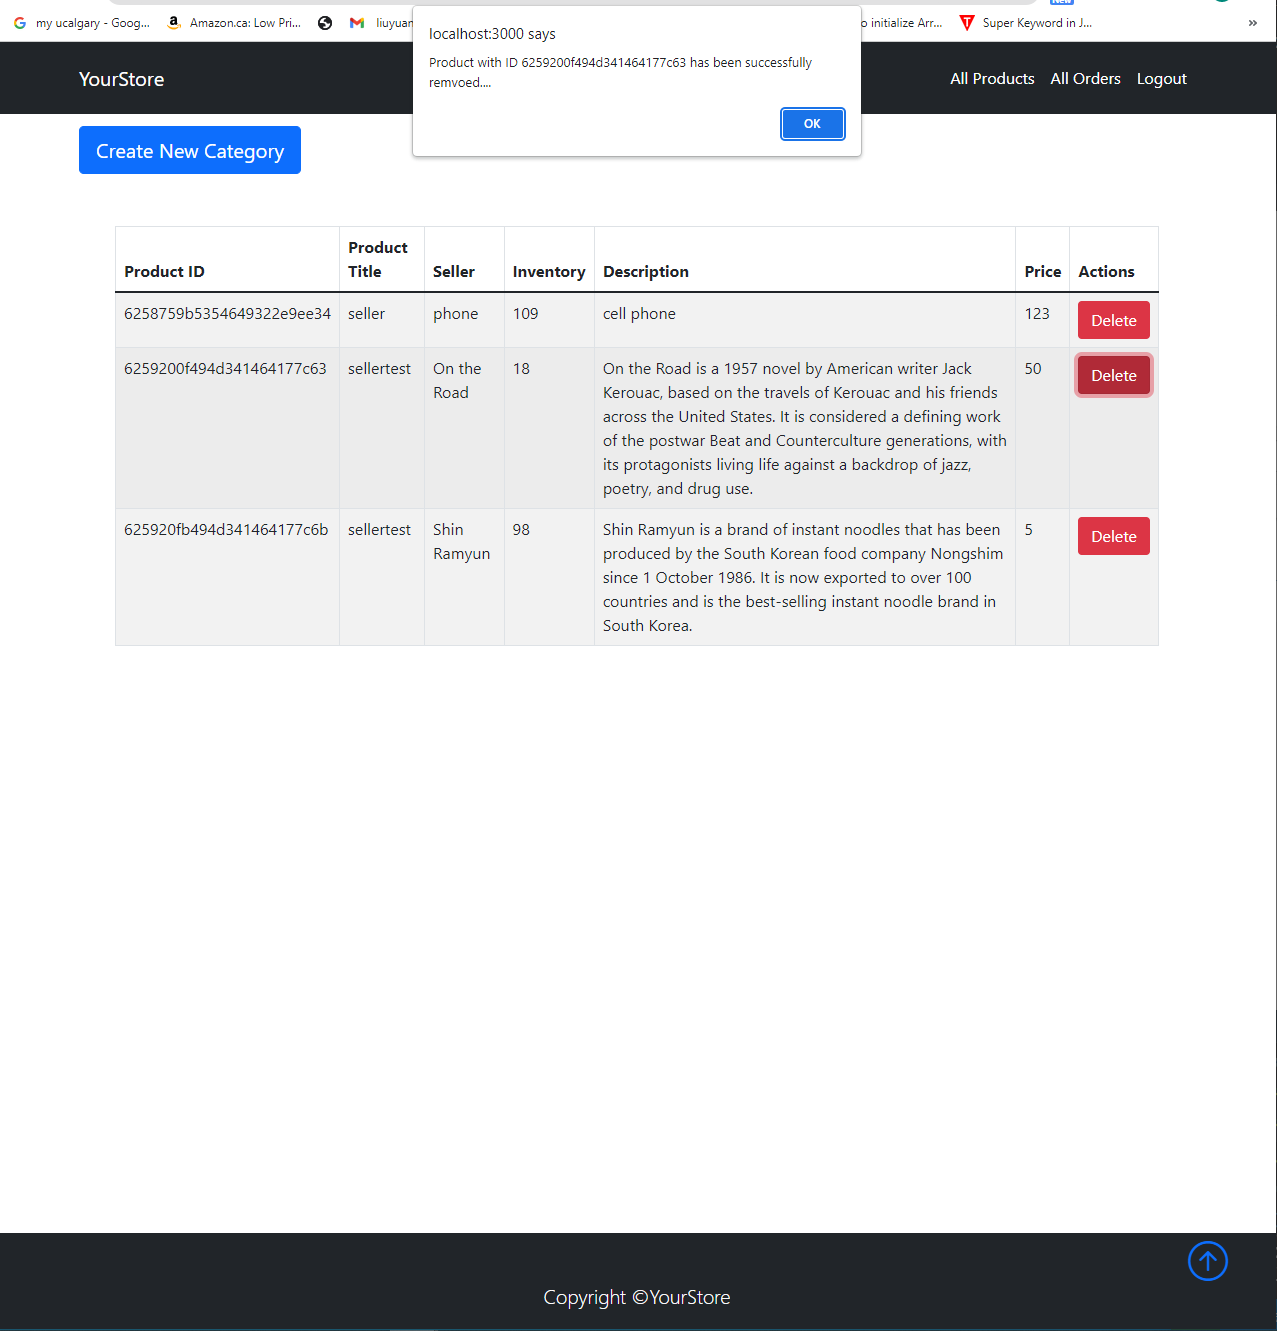
\includegraphics[width=0.45\textwidth]{UserGuideImage/4.png}

\vspace*{5mm}
\textbf{3: Admin manage orders}

Click “All Orders” on nav bar, admin can delete any existing orders as below.

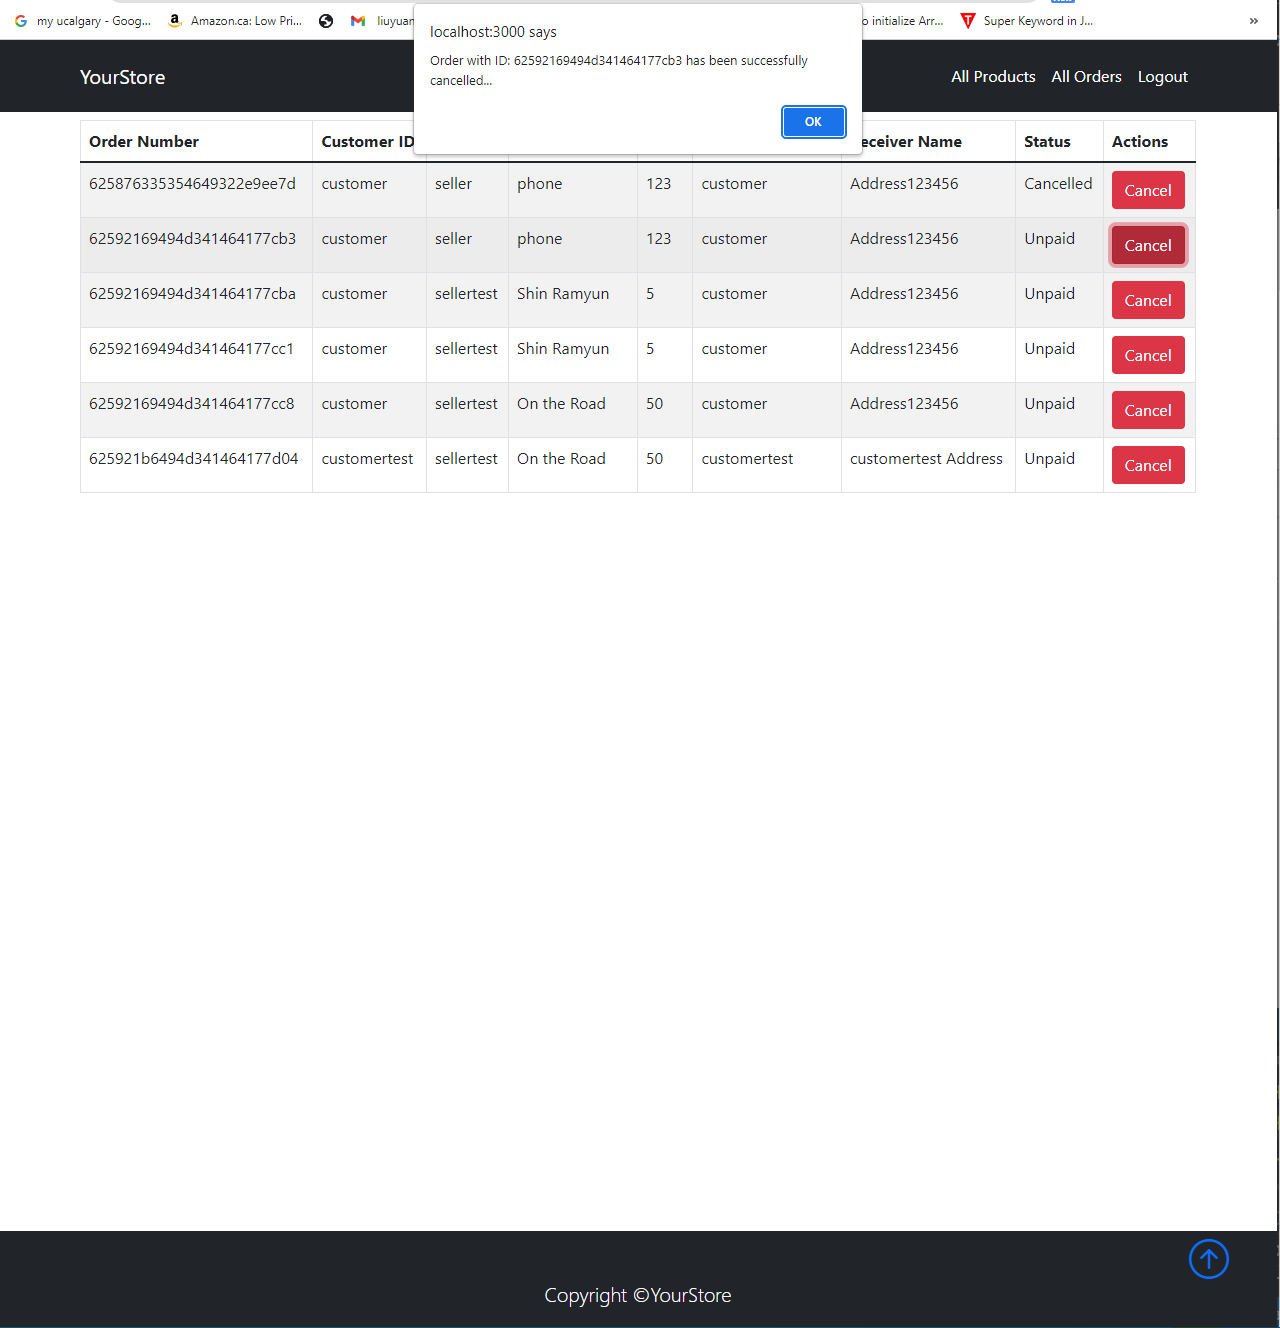
\includegraphics[width=0.45\textwidth]{UserGuideImage/5.png}

\newpage
\textbf{4: Sign in as seller}

Register a seller account and then sign in with the information that used for account registration.

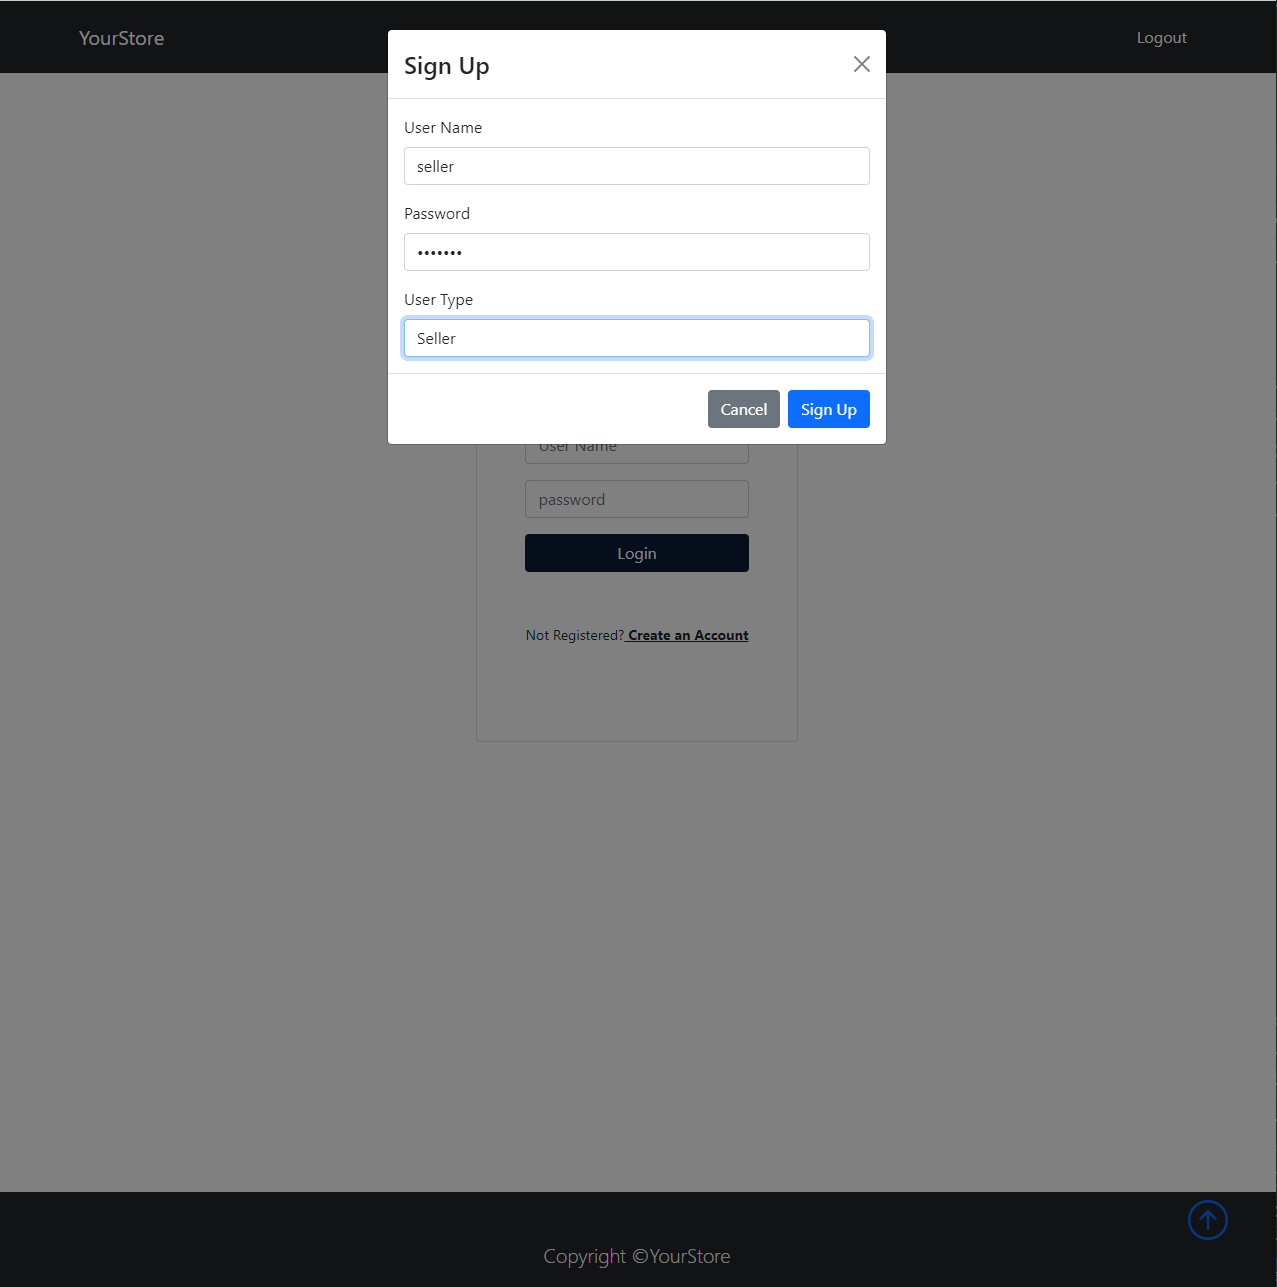
\includegraphics[width=0.45\textwidth]{UserGuideImage/6.png}
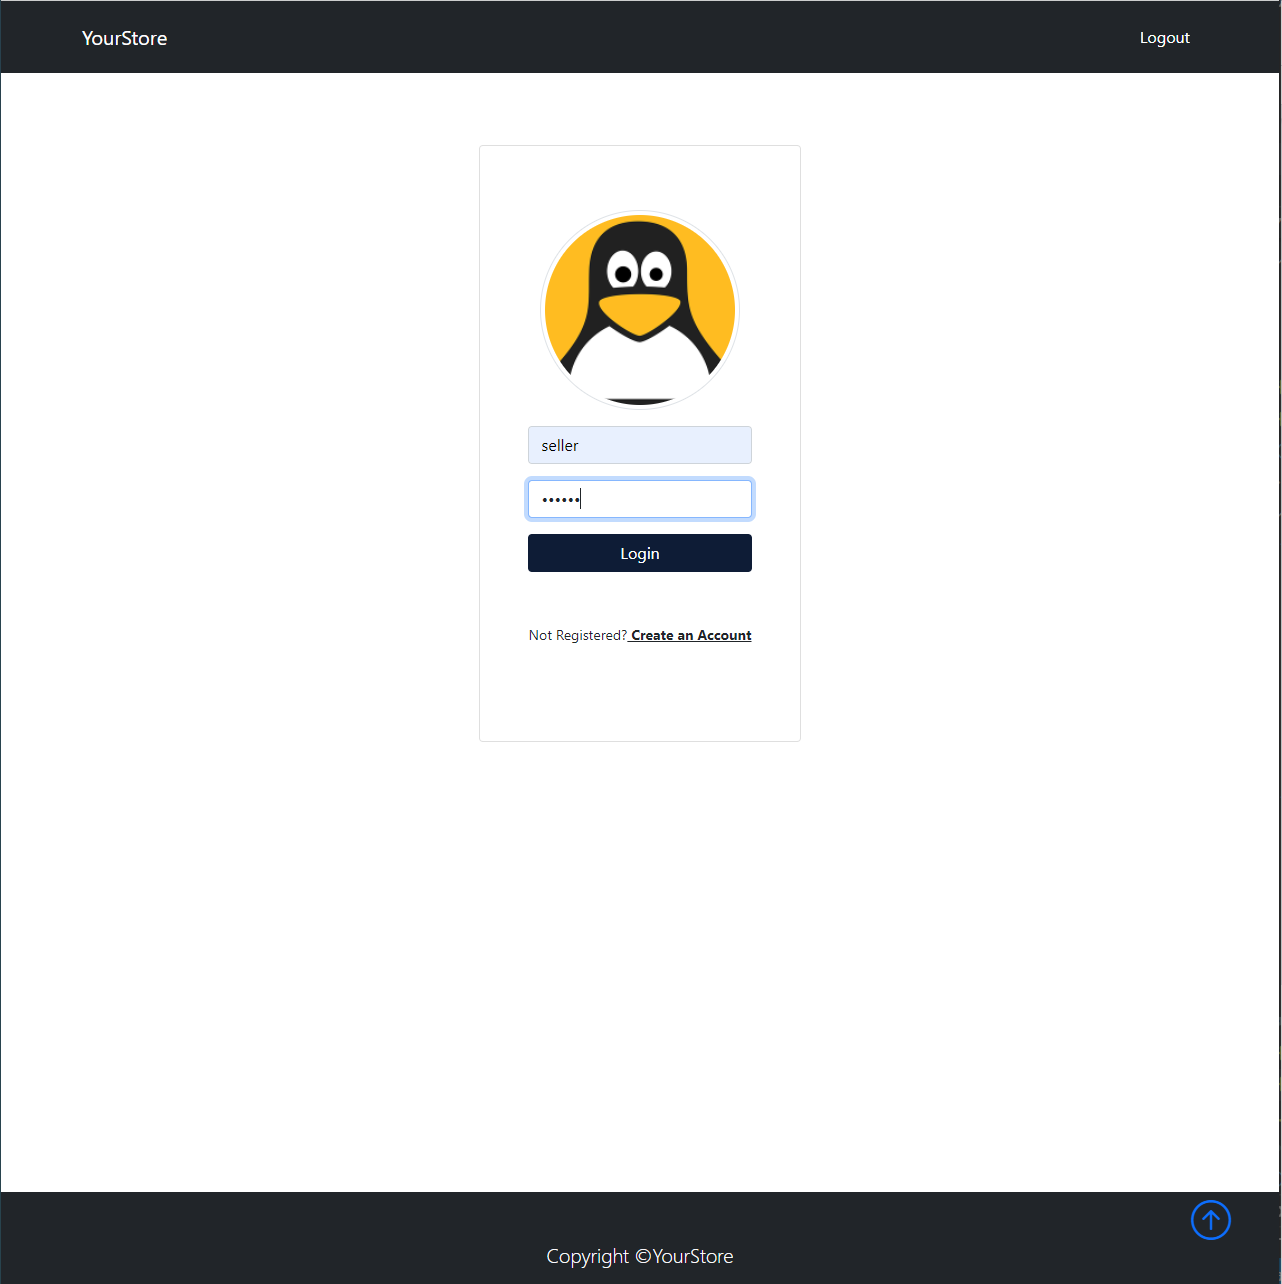
\includegraphics[width=0.45\textwidth]{UserGuideImage/7.png}


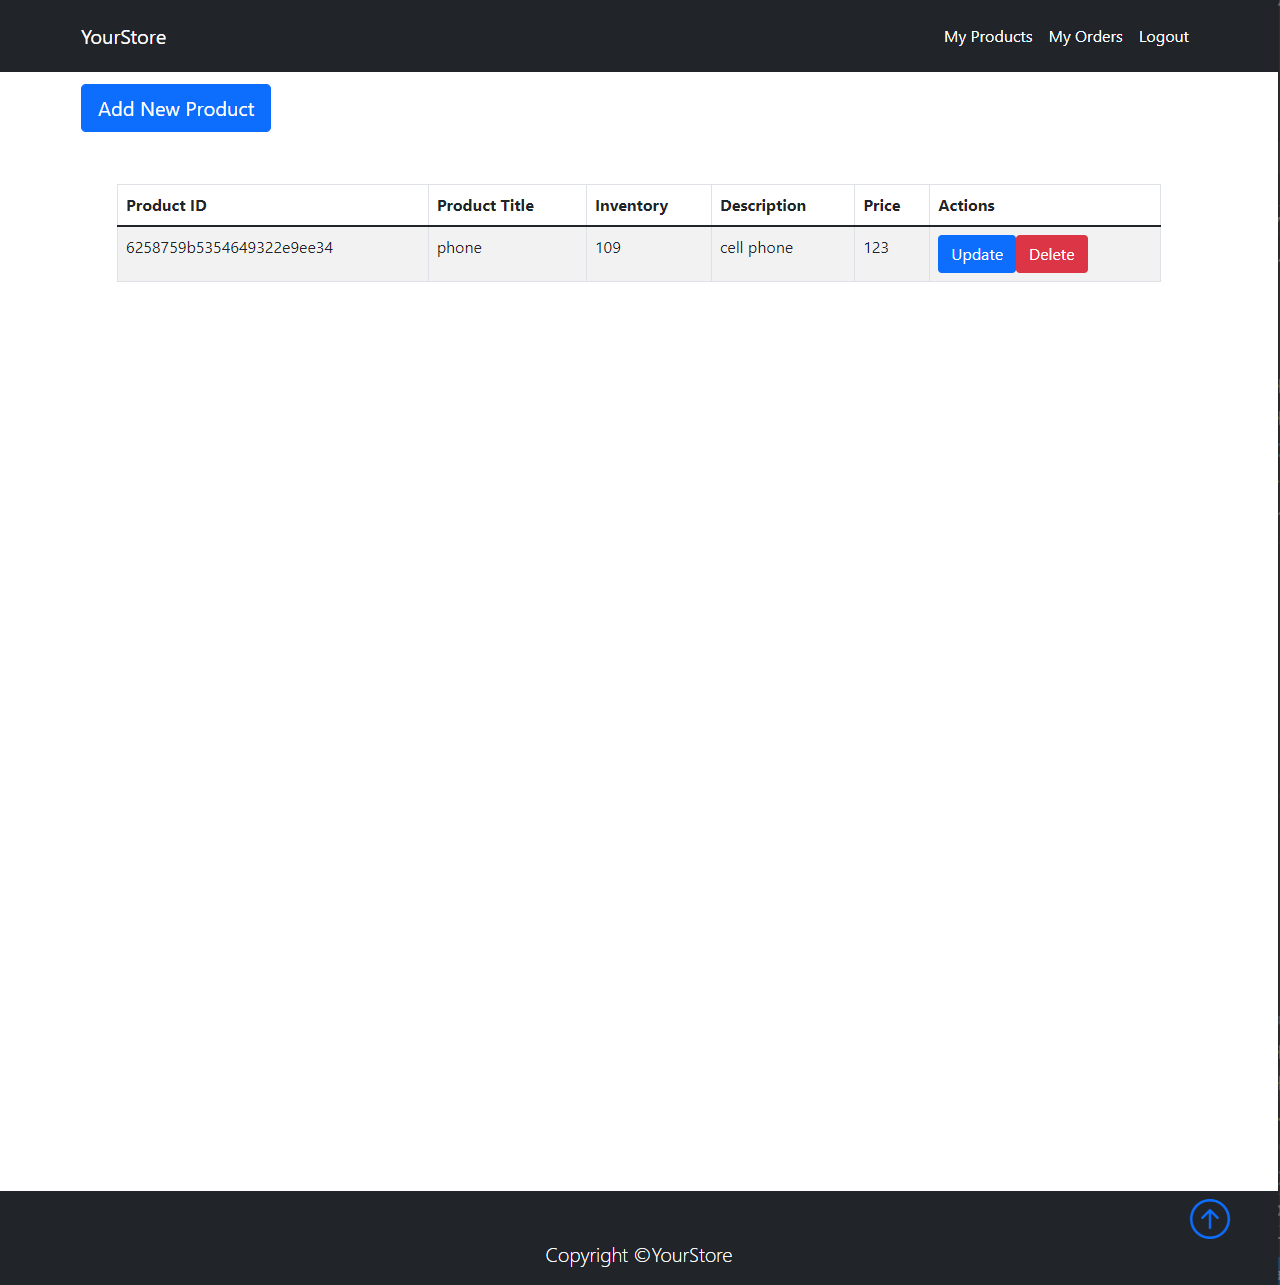
\includegraphics[width=0.45\textwidth]{UserGuideImage/8.png}

\newpage
\textbf{5: Seller manage products}

You can access “My Products” page by automatically sign in as seller or click “My Products”
at nav bar. In “My Products” page, seller can create a new product as below by clicking "Add New Product".

\vspace*{5mm}
\hspace*{5mm}\textbf{5.1: Create a new product}

Filled in all the blanked fields, and click "Create Product" to actually create the product.

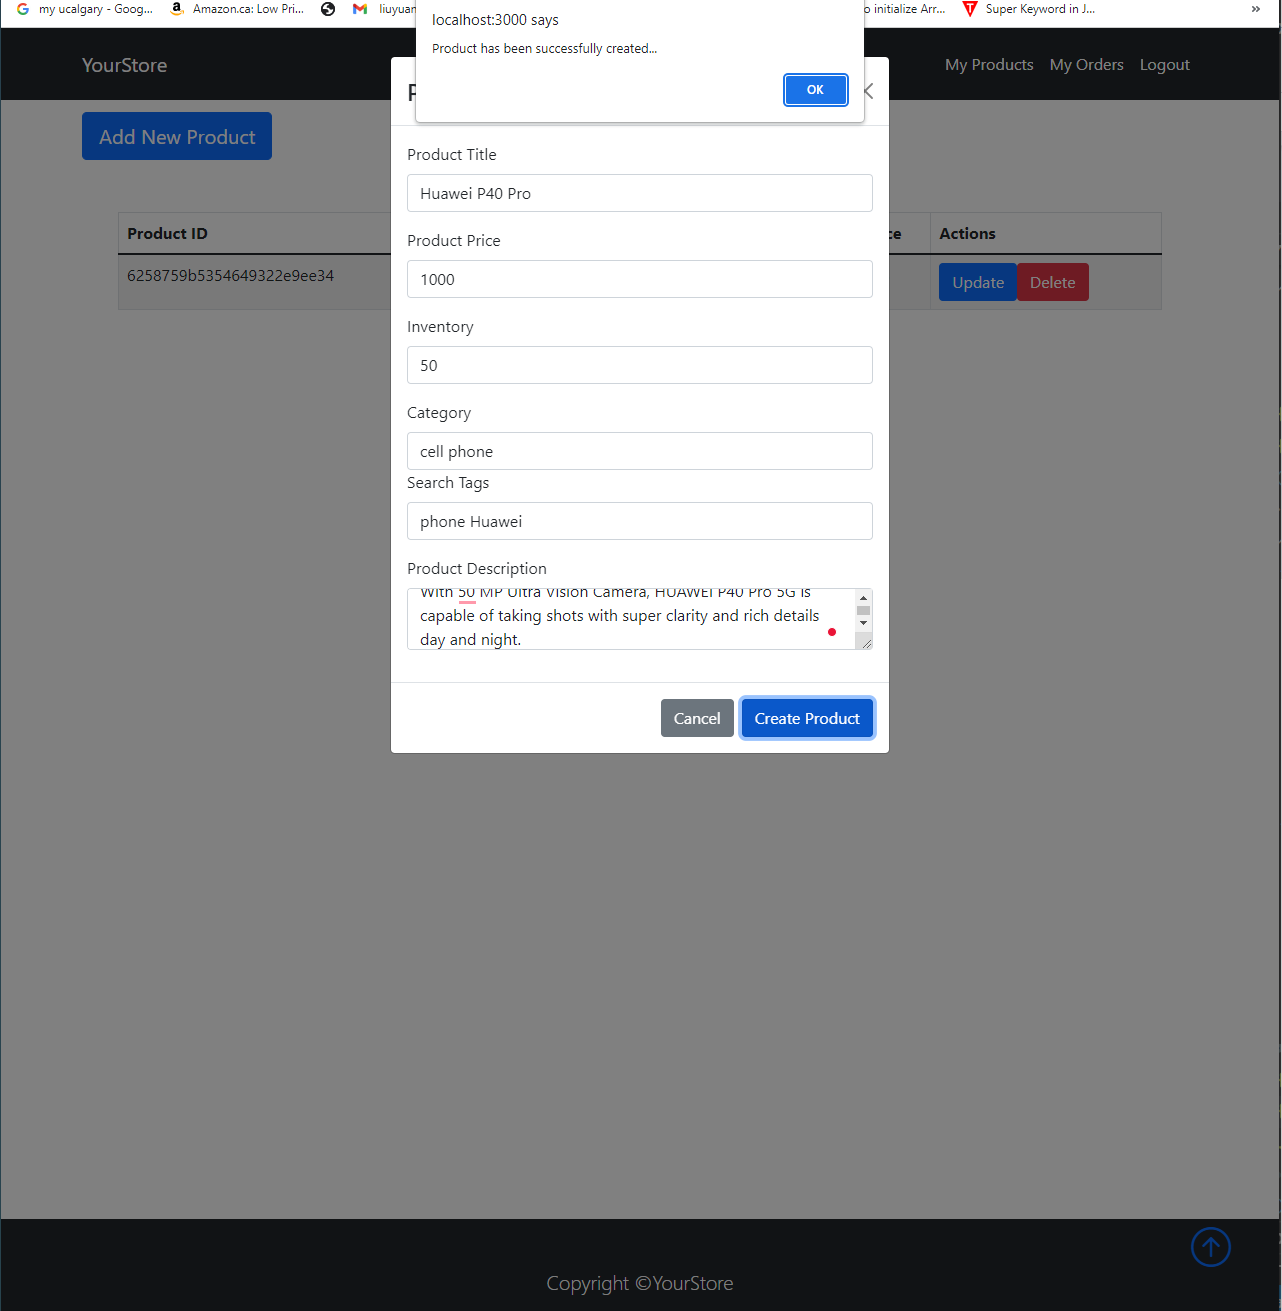
\includegraphics[width=0.45\textwidth]{UserGuideImage/9.png}

\vspace*{5mm}
\hspace*{5mm}\textbf{5.2: Update/Delete products}

You can choose to update or delete product by click corresponding buttons.

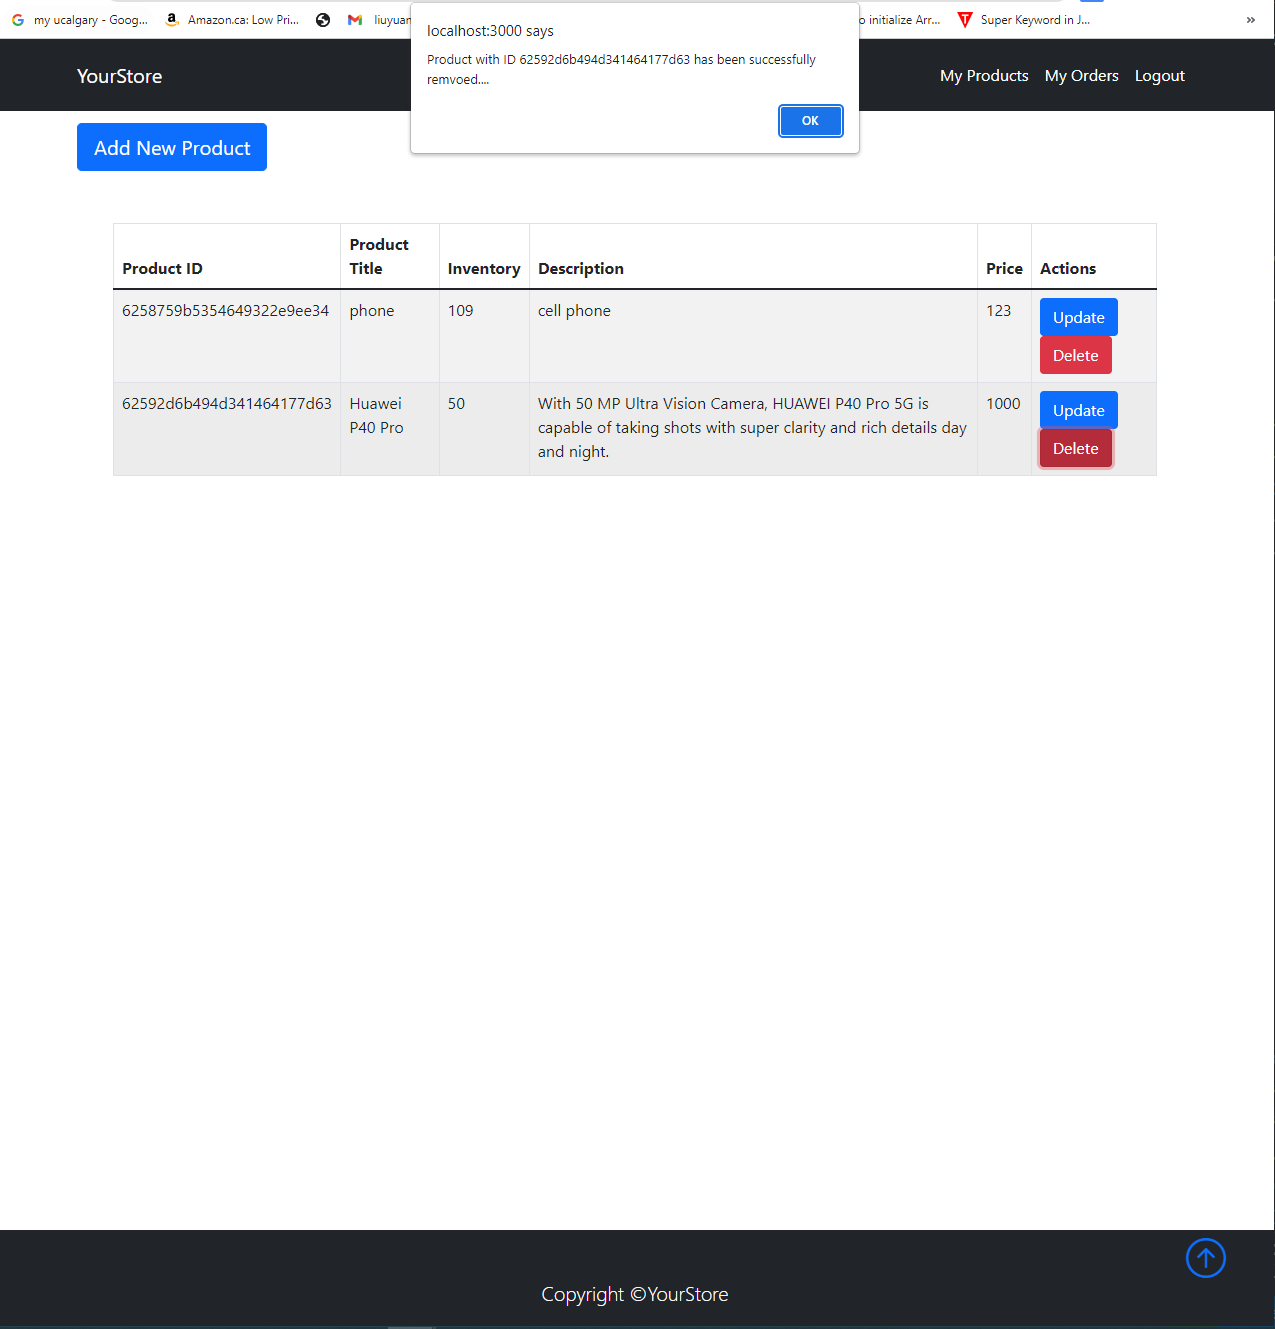
\includegraphics[width=0.45\textwidth]{UserGuideImage/10.png}

\newpage
\textbf{6: Seller manage orders}

Click “My Orders” on nav bar, seller can update/delete any existing orders as below.
Note that you only need to fill in the fields that need to be updated.

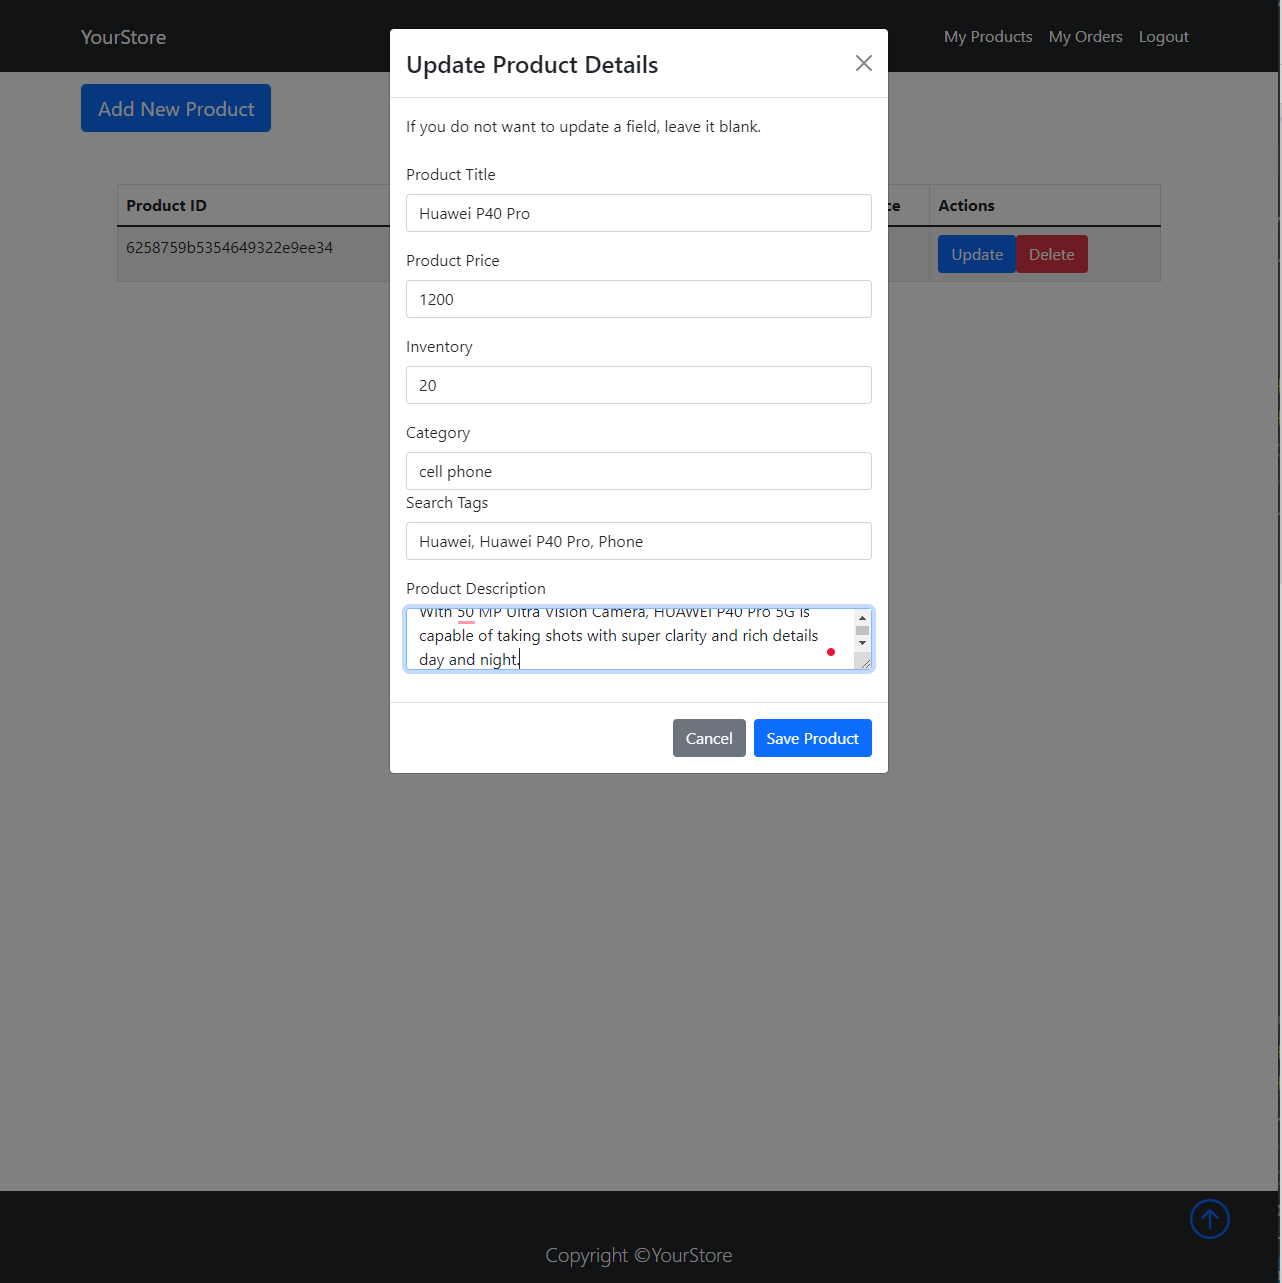
\includegraphics[width=0.45\textwidth]{UserGuideImage/11.png}


\newpage
\textbf{7: Sign in as customer}

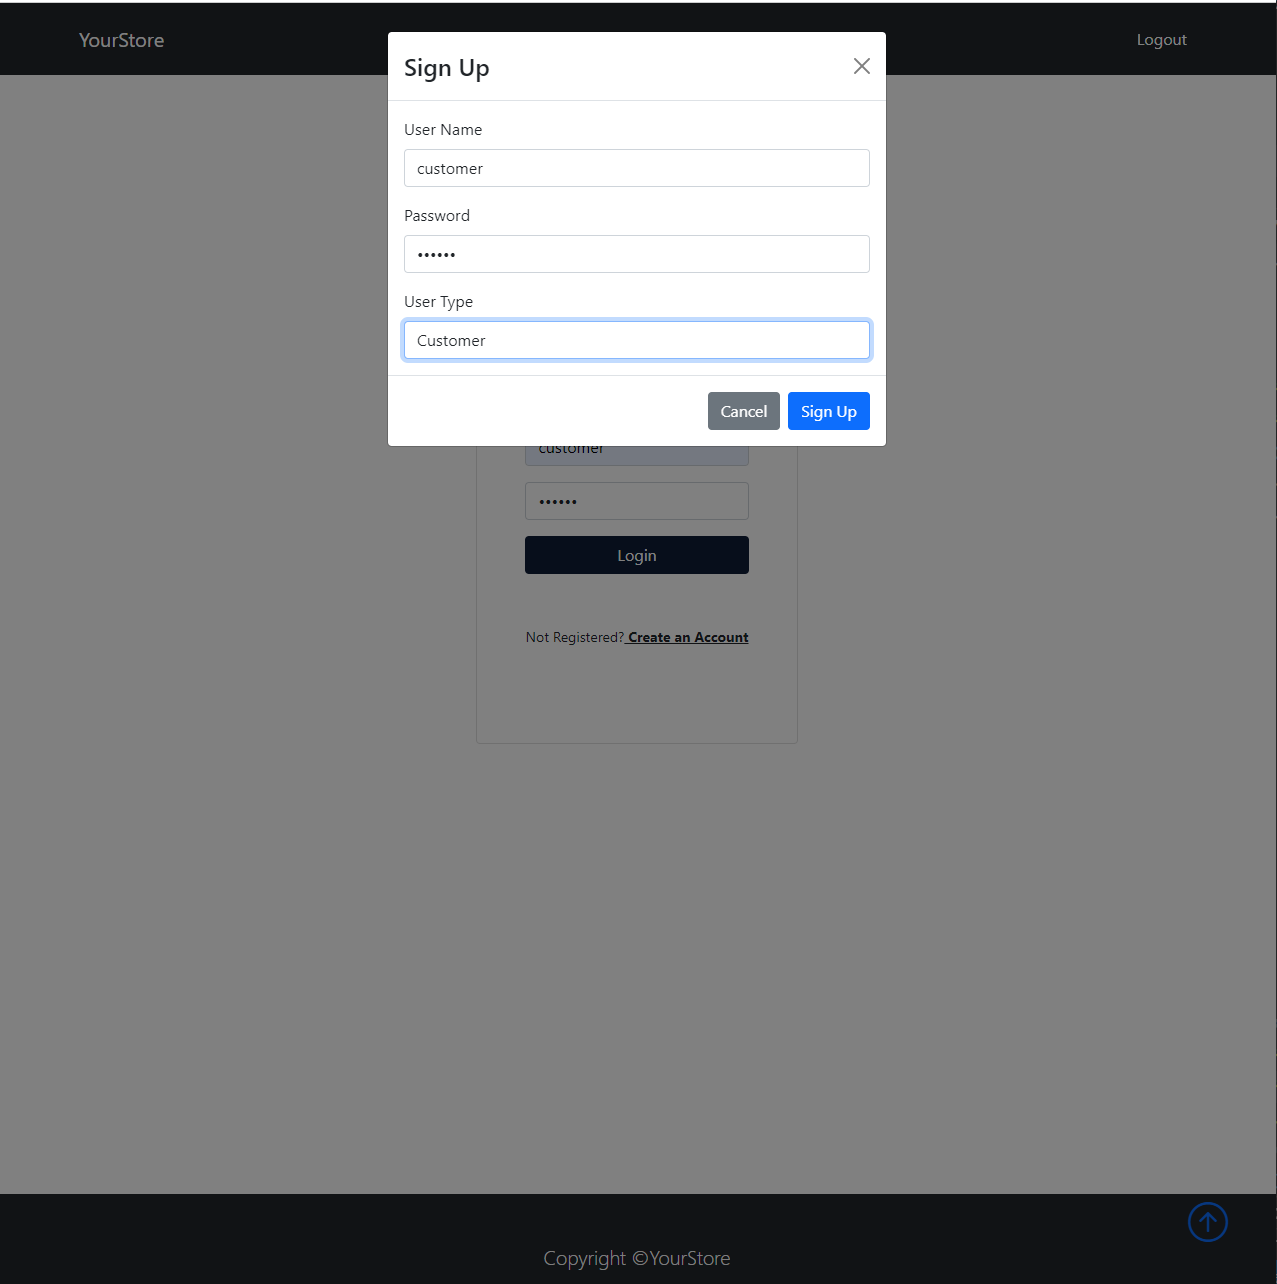
\includegraphics[width=0.45\textwidth]{UserGuideImage/12.png}
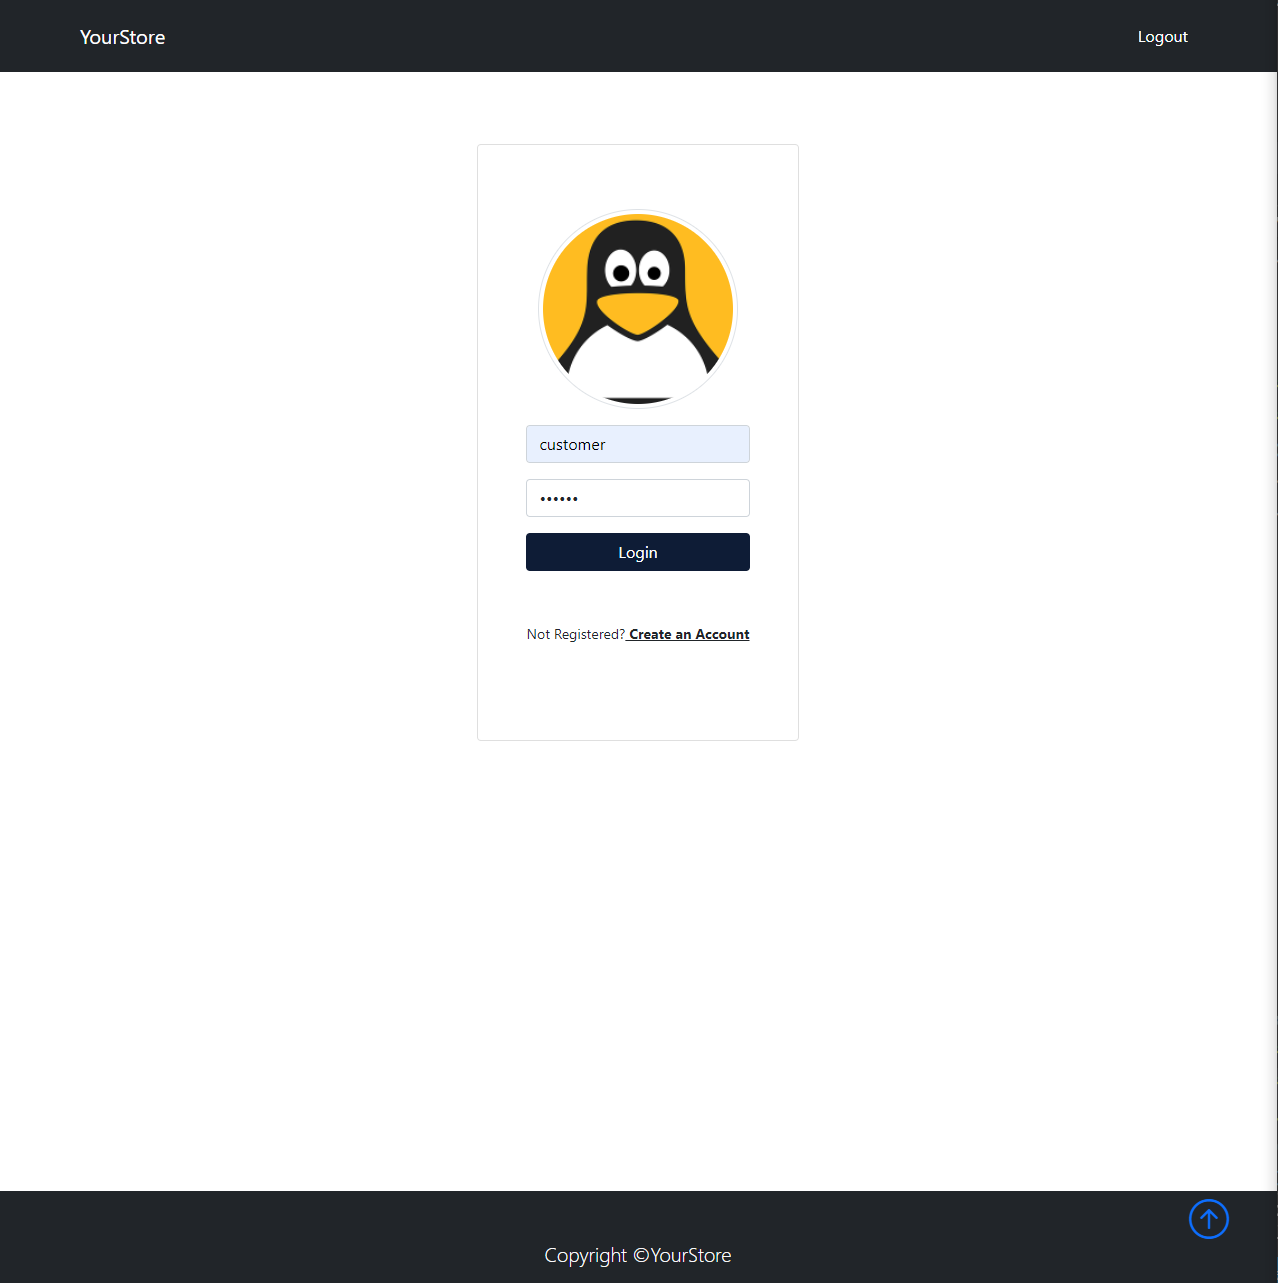
\includegraphics[width=0.45\textwidth]{UserGuideImage/13.png}

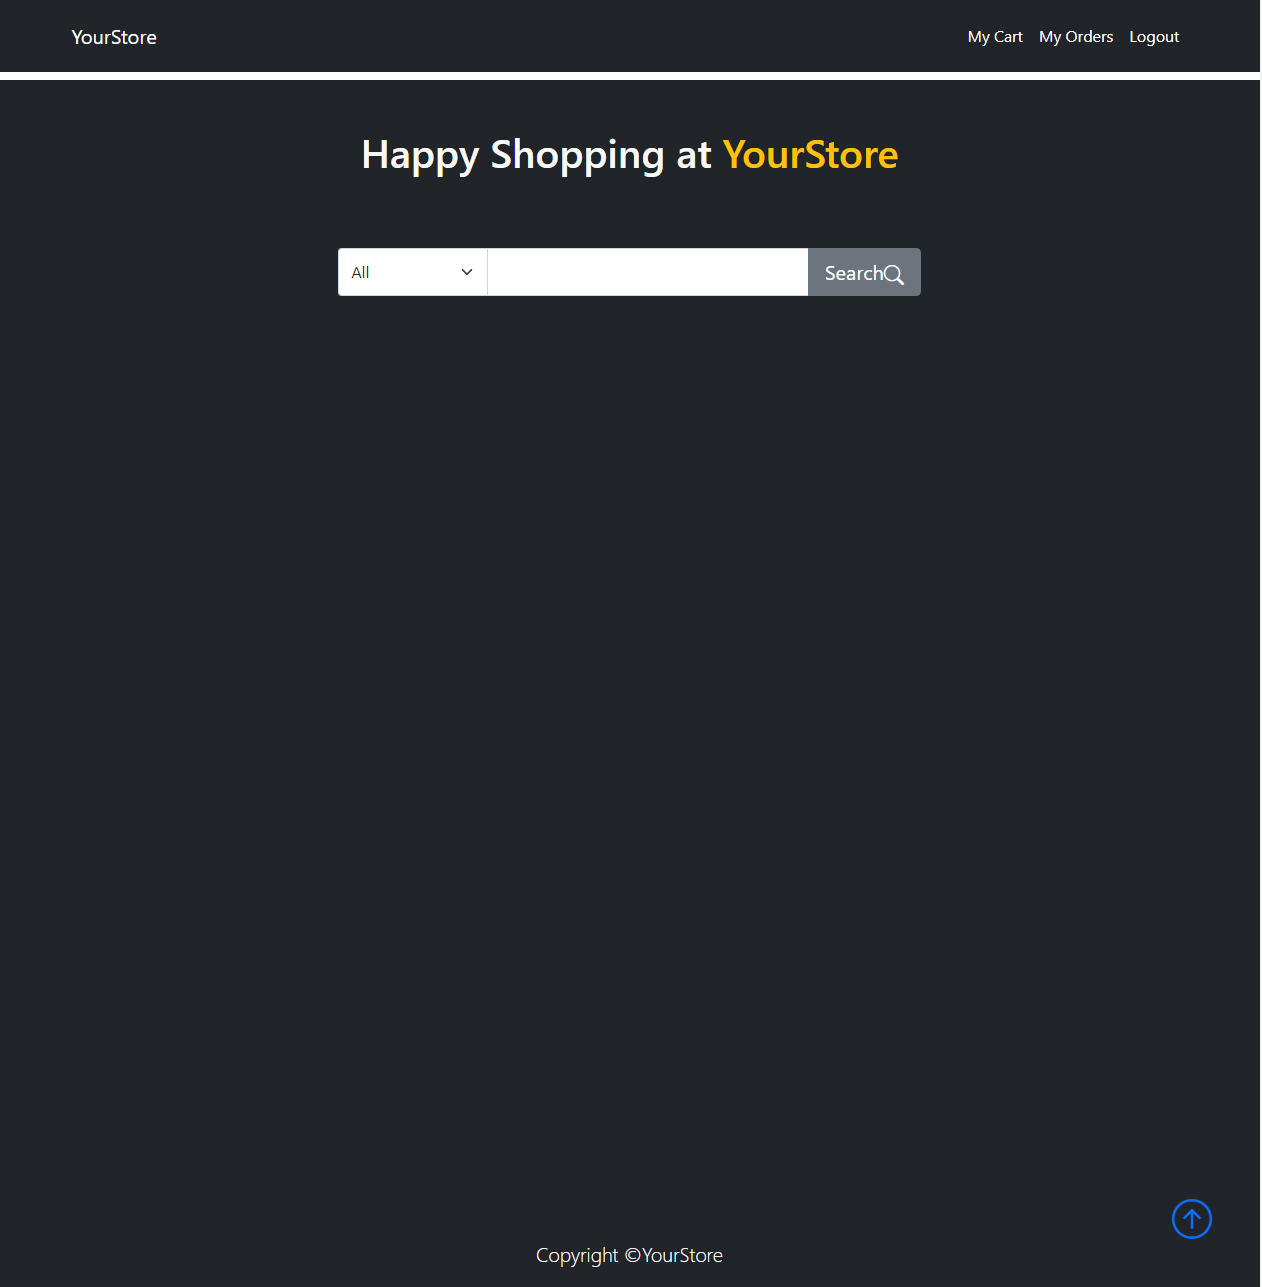
\includegraphics[width=0.45\textwidth]{UserGuideImage/14.png}

\newpage
\textbf{8: Customer add product to cart}

After searching the products, the customer can choose his/her favorite product and click "Add To Cart" button
to add the product into the cart.

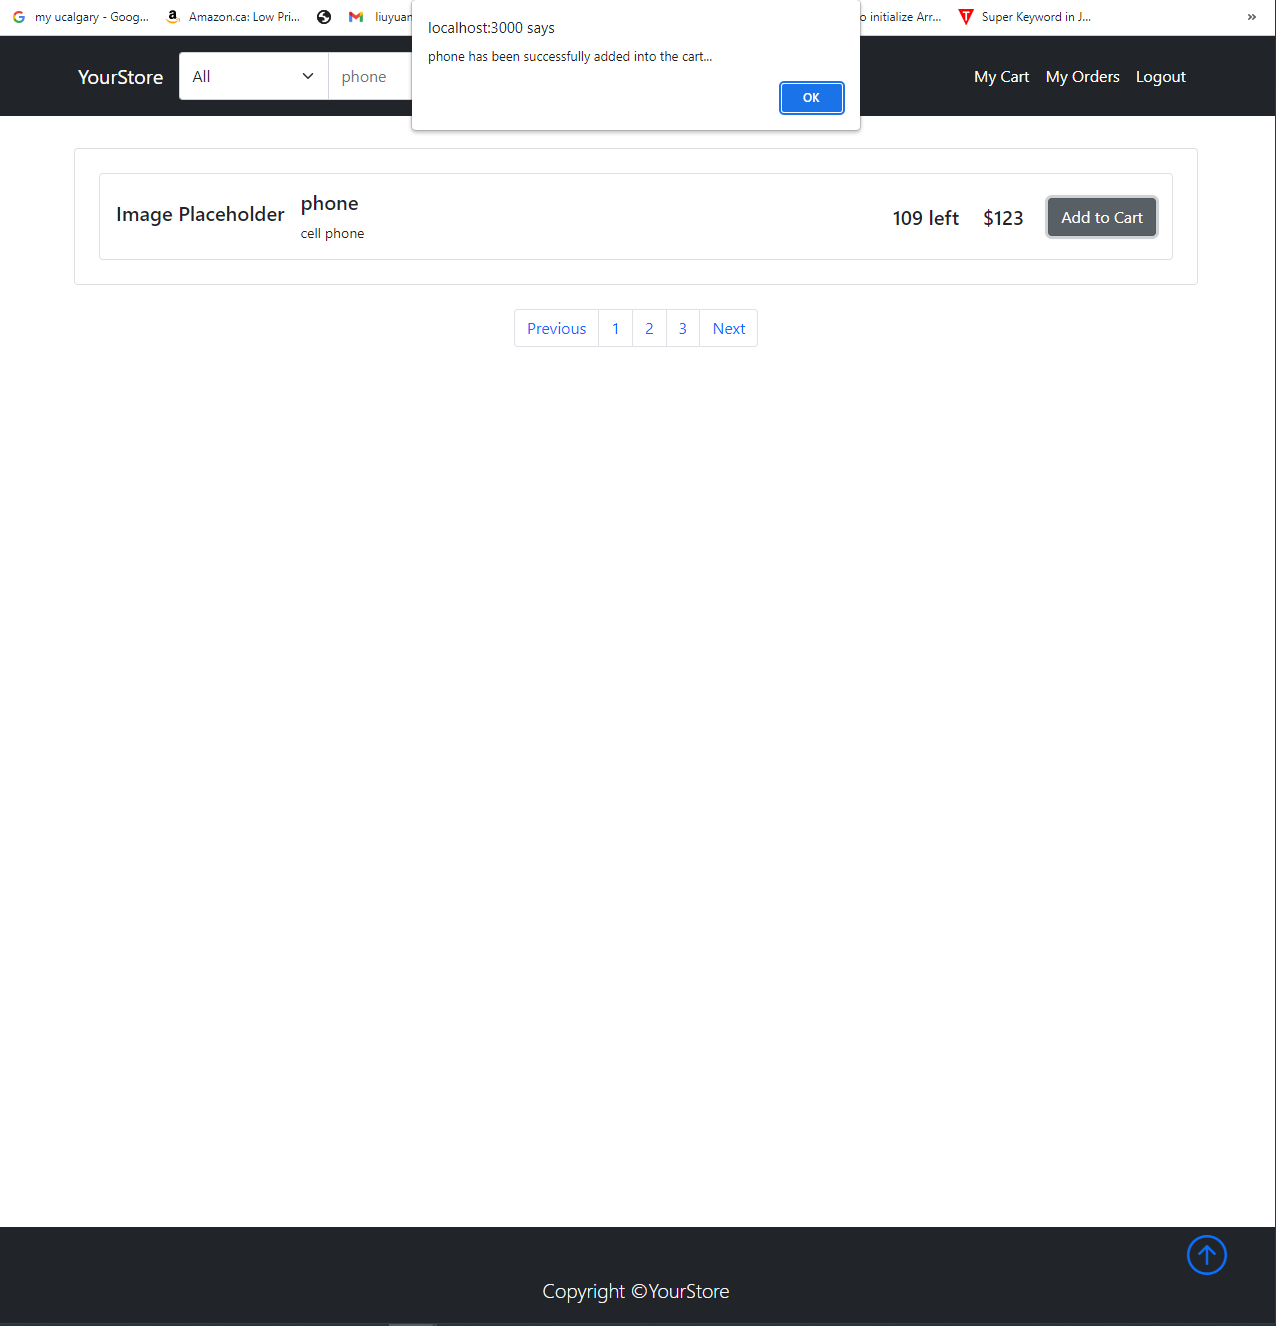
\includegraphics[width=0.45\textwidth]{UserGuideImage/15.png}

\vspace*{5mm}
\textbf{9: Customer place order}

The customer can navigate to his/her cart by clicking "My Cart" on the navigation bar. After examing 
the cart carefully, the customer can fill in the receiver details in the grey box and click "Purchase" to create orders.

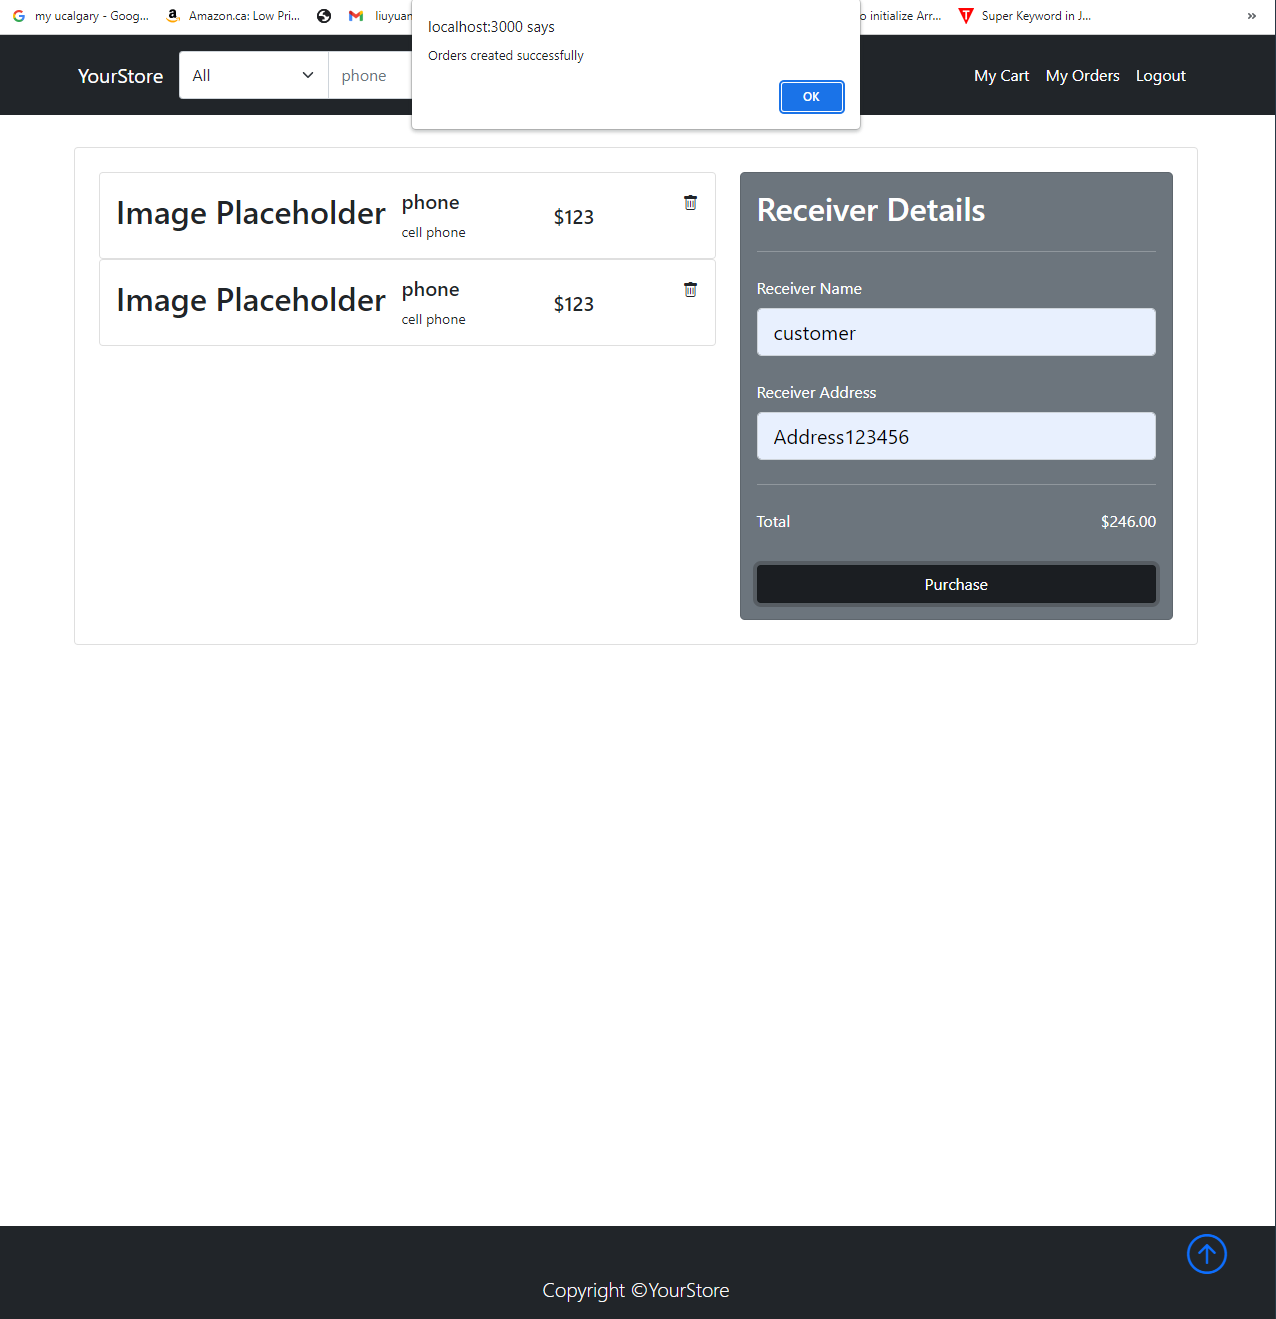
\includegraphics[width=0.45\textwidth]{UserGuideImage/16.png}

\newpage
\textbf{10: Customer manage order}

After click "My Orders" link in the navigation bar, the customer should be redirected to a page that he/she can manage 
his/her orders. The customer can choose to "Pay" for the order or "Cancel" the order by clicking 
the corresponding buttons.

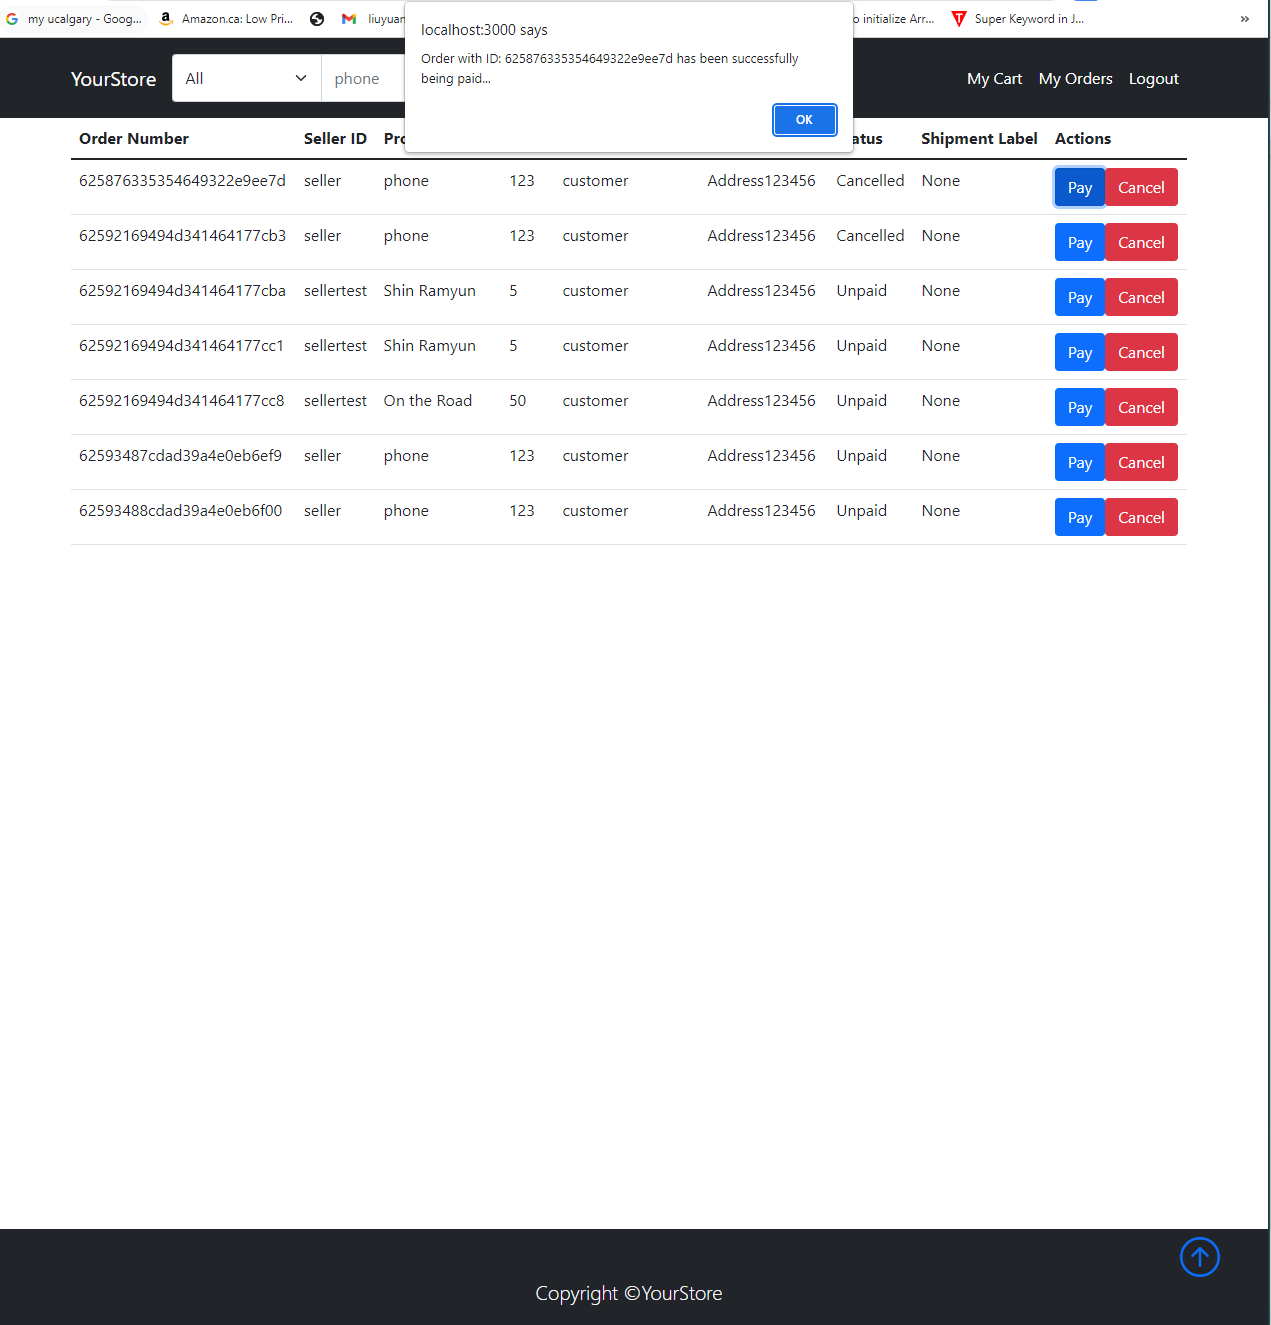
\includegraphics[width=0.45\textwidth]{UserGuideImage/17.png}


\end{document}